% This LaTeX document needs to be compiled with XeLaTeX.
\documentclass[10pt]{article}
\usepackage[utf8]{inputenc}
\usepackage{graphicx}
\usepackage[export]{adjustbox}
\graphicspath{ {./images/} }
\usepackage{amsmath}
\usepackage{amsfonts}
\usepackage{amssymb}
\usepackage[version=4]{mhchem}
\usepackage{stmaryrd}
\usepackage{multirow}
\usepackage[fallback]{xeCJK}
\usepackage{polyglossia}
\usepackage{fontspec}
\setCJKmainfont{Noto Serif CJK TC}

\setmainlanguage{polish}
\setmainfont{CMU Serif}

\title{EGZAMIN MATURALNY Z MATEMATYKI }

\author{}
\date{}


\begin{document}
\maketitle
\begin{center}

\includegraphics[max width=\textwidth]{2024_11_21_e0e8aab895018a50a9a7g-01}
\end{center}

POZIOM PODSTAWOWY\\
MAJ 2013

\begin{enumerate}
  \item Sprawdź, czy arkusz egzaminacyjny zawiera 22 strony (zadania 1-34). Ewentualny brak zgłoś przewodniczącemu zespołu nadzorującego egzamin.
  \item Rozwiązania zadań i odpowiedzi wpisuj w miejscu na to przeznaczonym.
  \item Odpowiedzi do zadań zamkniętych (1-25) przenieś na kartę odpowiedzi, zaznaczając je w części karty przeznaczonej dla zdającego. Zamaluj ■ pola do tego przeznaczone. Błędne zaznaczenie otocz kółkiem i zaznacz właściwe.
  \item Pamiętaj, że pominięcie argumentacji lub istotnych obliczeń w rozwiązaniu zadania otwartego (26-34) może spowodować, że za to rozwiązanie nie będziesz mógł
\end{enumerate}

Czas pracy:\\
170 minut\\
dostać pełnej liczby punktów.\\
5. Pisz czytelnie i używaj tylko długopisu lub pióra z czarnym tuszem lub atramentem.\\
6. Nie używaj korektora, a błędne zapisy wyraźnie przekreśl.\\
7. Pamiętaj, że zapisy w brudnopisie nie będą oceniane.\\
8. Możesz korzystać z zestawu wzorów matematycznych, cyrkla i linijki oraz kalkulatora.\\
9. Na tej stronie oraz na karcie odpowiedzi wpisz swój numer PESEL i przyklej naklejkę z kodem.\\
10. Nie wpisuj żadnych znaków w części przeznaczonej dla egzaminatora.

Liczba punktów do uzyskania: 50

MMA-P1\_1P-132

\section*{ZADANIA ZAMKNIĘTE}
\section*{W zadaniach 1-25 wybierz i zaznacz na karcie odpowiedzi poprawnq odpowiedź.}
\section*{Zadanie 1. (1 pkt)}
Wskaż rysunek, na którym zaznaczony jest zbiór wszystkich liczb rzeczywistych spełniających nierówność \(|x+4|<5\).\\
A.\\
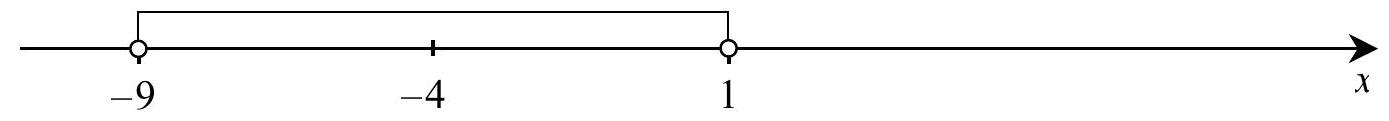
\includegraphics[max width=\textwidth, center]{2024_11_21_e0e8aab895018a50a9a7g-02(3)}\\
B.\\
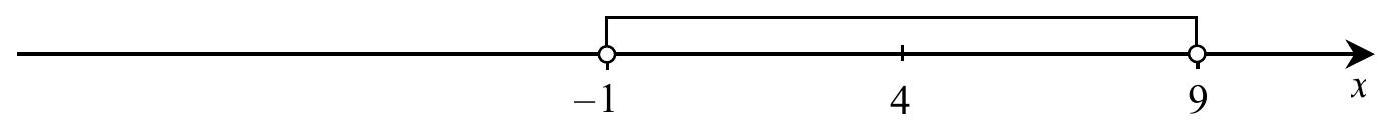
\includegraphics[max width=\textwidth, center]{2024_11_21_e0e8aab895018a50a9a7g-02(2)}\\
C.\\
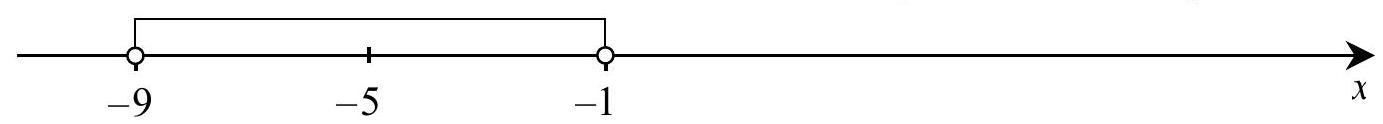
\includegraphics[max width=\textwidth, center]{2024_11_21_e0e8aab895018a50a9a7g-02}\\
D.\\
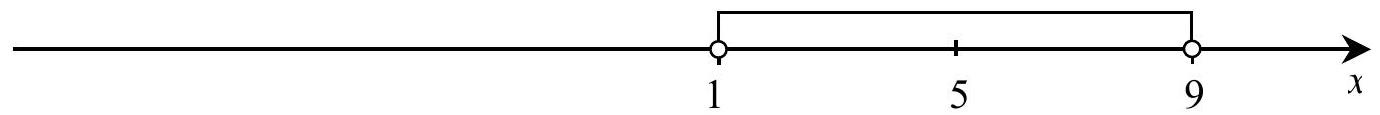
\includegraphics[max width=\textwidth, center]{2024_11_21_e0e8aab895018a50a9a7g-02(1)}

\section*{Zadanie 2. (1 pkt)}
Liczby \(a\) i \(b\) są dodatnie oraz \(12 \%\) liczby \(a\) jest równe \(15 \%\) liczby \(b\). Stąd wynika, że \(a\) jest równe\\
A. \(103 \%\) liczby \(b\)\\
B. \(125 \%\) liczby \(b\)\\
C. \(150 \%\) liczby \(b\)\\
D. \(153 \%\) liczby \(b\)

\section*{Zadanie 3. (1 pkt)}
Liczba \(\log 100-\log _{2} 8\) jest równa\\
A. -2\\
B. -1\\
C. 0\\
D. 1

\section*{Zadanie 4. (1 pkt)}
Rozwiązaniem układu równań \(\left\{\begin{array}{l}5 x+3 y=3 \\ 8 x-6 y=48\end{array}\right.\) jest para liczb\\
A. \(x=-3\) i \(y=4\)\\
B. \(x=-3\) i \(y=6\)\\
C. \(x=3\) i \(y=-4\)\\
D. \(x=9\) i \(y=4\)

\section*{Zadanie 5. (1 pkt)}
Punkt \(A=(0,1)\) leży na wykresie funkcji liniowej \(f(x)=(m-2) x+m-3\). Stąd wynika, że\\
A. \(m=1\)\\
B. \(m=2\)\\
C. \(m=3\)\\
D. \(m=4\)

\section*{Zadanie 6. (1 pkt)}
Wierzchołkiem paraboli o równaniu \(y=-3(x-2)^{2}+4\) jest punkt o współrzędnych\\
A. \((-2,-4)\)\\
B. \((-2,4)\)\\
C. \((2,-4)\)\\
D. \((2,4)\)

\section*{Zadanie 7. (1 pkt)}
Dla każdej liczby rzeczywistej \(x\), wyrażenie \(4 x^{2}-12 x+9\) jest równe\\
A. \((4 x+3)(x+3)\)\\
B. \((2 x-3)(2 x+3)\)\\
C. \((2 x-3)(2 x-3)\)\\
D. \((x-3)(4 x-3)\)

\section*{BRUDNOPIS}
\begin{center}

\includegraphics[max width=\textwidth]{2024_11_21_e0e8aab895018a50a9a7g-03}
\end{center}

\section*{Zadanie 8. (1 pkt)}
Prosta o równaniu \(y=\frac{2}{m} x+1\) jest prostopadła do prostej o równaniu \(y=-\frac{3}{2} x-1\). Stąd wynika, że\\
A. \(m=-3\)\\
B. \(m=\frac{2}{3}\)\\
C. \(m=\frac{3}{2}\)\\
D. \(m=3\)

\section*{Zadanie 9. (1 pkt)}
Na rysunku przedstawiony jest fragment wykresu pewnej funkcji liniowej \(y=a x+b\).\\
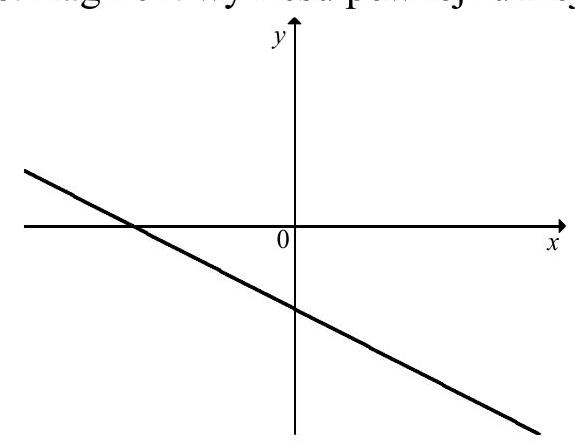
\includegraphics[max width=\textwidth, center]{2024_11_21_e0e8aab895018a50a9a7g-04(1)}

Jakie znaki mają współczynniki \(a\) i \(b\) ?\\
A. \(a<0\) i \(b<0\)\\
B. \(a<0\) i \(b>0\)\\
C. \(a>0\) i \(b<0\)\\
D. \(a>0\) i \(b>0\)

\section*{Zadanie 10. (1 pkt)}
Najmniejszą liczbą całkowitą spełniającą nierówność \(\frac{x}{2} \leq \frac{2 x}{3}+\frac{1}{4}\) jest\\
A. -2\\
B. -1\\
C. 0\\
D. 1

\section*{Zadanie 11. (1 pkt)}
Na rysunku 1 przedstawiony jest wykres funkcji \(y=f(x)\) określonej dla \(x \in\langle-7,4\rangle\).\\
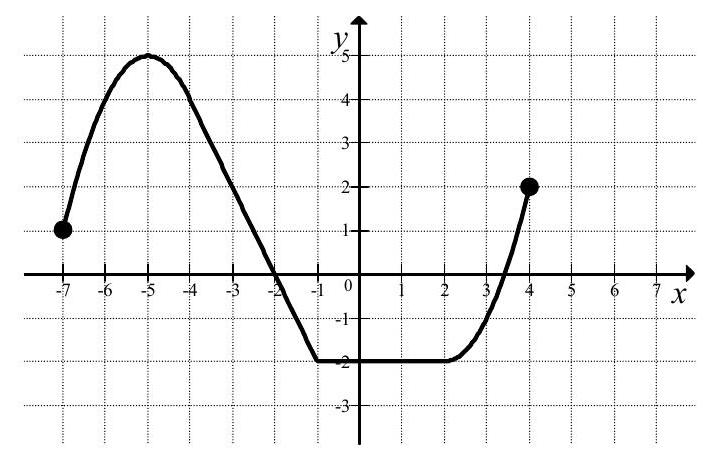
\includegraphics[max width=\textwidth, center]{2024_11_21_e0e8aab895018a50a9a7g-04(2)}

Rys. 1\\
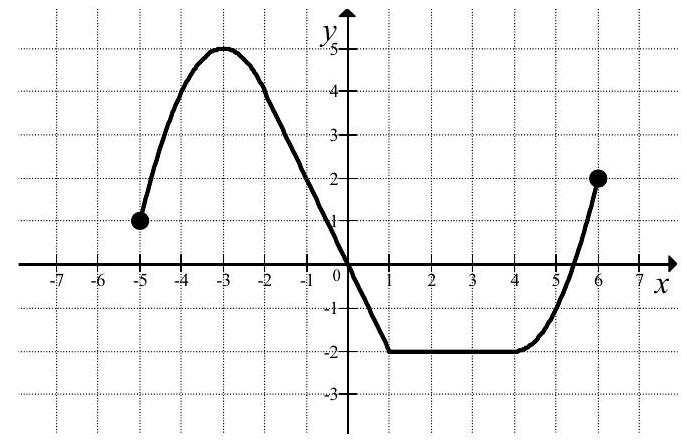
\includegraphics[max width=\textwidth, center]{2024_11_21_e0e8aab895018a50a9a7g-04}

Rys. 2

Rysunek 2 przedstawia wykres funkcji\\
A. \(y=f(x+2)\)\\
B. \(y=f(x)-2\)\\
C. \(y=f(x-2)\)\\
D. \(y=f(x)+2\)

Zadanie 12. (1 pkt)\\
Caag \((27,18, x+5)\) jest geometryczny. Wtedy\\
A. \(x=4\)\\
B. \(x=5\)\\
C. \(x=7\)\\
D. \(x=9\)

\section*{BRUDNOPIS}
\begin{center}

\includegraphics[max width=\textwidth]{2024_11_21_e0e8aab895018a50a9a7g-05}
\end{center}

\section*{Zadanie 13. (1 pkt)}
Caag \(\left(a_{n}\right)\) określony dla \(n \geq 1\) jest arytmetyczny oraz \(a_{3}=10\) i \(a_{4}=14\). Pierwszy wyraz tego ciagu jest równy\\
A. \(a_{1}=-2\)\\
B. \(a_{1}=2\)\\
C. \(a_{1}=6\)\\
D. \(a_{1}=12\)

\section*{Zadanie 14. (1 pkt)}
Kąt \(\alpha\) jest ostry i \(\sin \alpha=\frac{\sqrt{3}}{2}\). Wartość wyrażenia \(\cos ^{2} \alpha-2\) jest równa\\
A. \(-\frac{7}{4}\)\\
B. \(-\frac{1}{4}\)\\
C. \(\frac{1}{2}\)\\
D. \(\frac{\sqrt{3}}{2}\)

\section*{Zadanie 15. (1 pkt)}
Średnice \(A B\) i \(C D\) okręgu o środku \(S\) przecinają się pod kątem \(50^{\circ}\) (tak jak na rysunku).\\
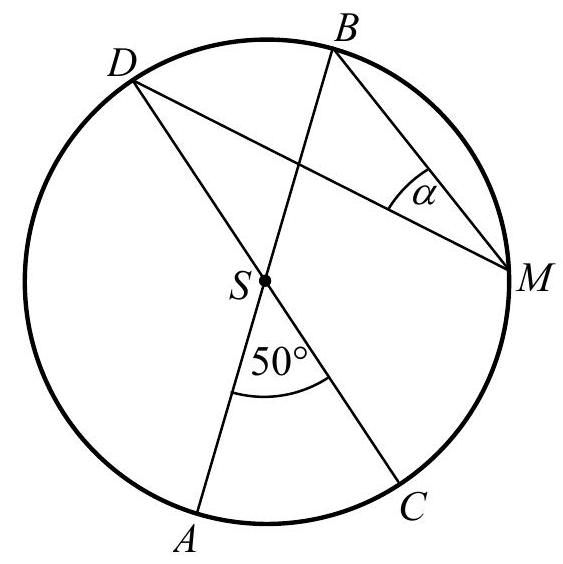
\includegraphics[max width=\textwidth, center]{2024_11_21_e0e8aab895018a50a9a7g-06}

Miara kąta \(\alpha\) jest równa\\
A. \(25^{\circ}\)\\
B. \(30^{\circ}\)\\
C. \(40^{\circ}\)\\
D. \(50^{\circ}\)

\section*{Zadanie 16. (1 pkt)}
Liczba rzeczywistych rozwiązań równania \((x+1)(x+2)\left(x^{2}+3\right)=0\) jest równa\\
A. 0\\
B. 1\\
C. 2\\
D. 4

\section*{Zadanie 17. (1 pkt)}
Punkty \(A=(-1,2)\) i \(B=(5,-2)\) są dwoma sąsiednimi wierzchołkami rombu \(A B C D\). Obwód tego rombu jest równy\\
A. \(\sqrt{13}\)\\
B. 13\\
C. 676\\
D. \(8 \sqrt{13}\)

Zadanie 18. (1 pkt)\\
Punkt \(S=(-4,7)\) jest środkiem odcinka \(P Q\), gdzie \(Q=(17,12)\). Zatem punkt \(P\) ma współrzędne\\
A. \(P=(2,-25)\)\\
B. \(P=(38,17)\)\\
C. \(P=(-25,2)\)\\
D. \(P=(-12,4)\)

\section*{BRUDNOPIS}
\begin{center}

\includegraphics[max width=\textwidth]{2024_11_21_e0e8aab895018a50a9a7g-07}
\end{center}

\section*{Zadanie 19. (1 pkt)}
Odległość między środkami okręgów o równaniach \((x+1)^{2}+(y-2)^{2}=9\) oraz \(x^{2}+y^{2}=10\) jest równa\\
A. \(\sqrt{5}\)\\
B. \(\sqrt{10}-3\)\\
C. 3\\
D. 5

\section*{Zadanie 20. (1 pkt)}
Liczba wszystkich krawędzi graniastosłupa jest o 10 większa od liczby wszystkich jego ścian bocznych. Stąd wynika, że podstawą tego graniastosłupa jest\\
A. czworokąt\\
B. pięciokąt\\
C. sześciokąt\\
D. dziesięciokąt

\section*{Zadanie 21. (1 pkt)}
Pole powierzchni bocznej stożka o wysokości 4 i promieniu podstawy 3 jest równe\\
A. \(9 \pi\)\\
B. \(12 \pi\)\\
C. \(15 \pi\)\\
D. \(16 \pi\)

\section*{Zadanie 22. (1 pkt)}
Rzucamy dwa razy symetryczną sześcienną kostka do gry. Niech \(p\) oznacza prawdopodobieństwo zdarzenia, że iloczyn liczb wyrzuconych oczek jest równy 5 . Wtedy\\
A. \(p=\frac{1}{36}\)\\
B. \(p=\frac{1}{18}\)\\
C. \(p=\frac{1}{12}\)\\
D. \(p=\frac{1}{9}\)

\section*{Zadanie 23. (1 pkt)}
Liczba \(\frac{\sqrt{50}-\sqrt{18}}{\sqrt{2}}\) jest równa\\
A. \(2 \sqrt{2}\)\\
B. 2\\
C. 4\\
D. \(\sqrt{10}-\sqrt{6}\)

\section*{Zadanie 24. (1 pkt)}
Mediana uporządkowanego niemalejąco zestawu sześciu liczb: \(1,2,3, x, 5,8\) jest równa 4. Wtedy\\
A. \(x=2\)\\
B. \(x=3\)\\
C. \(x=4\)\\
D. \(x=5\)

\section*{Zadanie 25. (1 pkt)}
Objętość graniastosłupa prawidłowego trójkątnego o wysokości 7 jest równa \(28 \sqrt{3}\). Długość krawędzi podstawy tego graniastosłupa jest równa\\
A. 2\\
B. 4\\
C. 8\\
D. 16

\section*{BRUDNOPIS}
\begin{center}

\includegraphics[max width=\textwidth]{2024_11_21_e0e8aab895018a50a9a7g-09}
\end{center}

\section*{ZADANIA OTWARTE}
\section*{Rozwiazzania zadań 26-34 nalè̇y zapisać \(\mathbf{w}\) wyznaczonych miejscach pod treścia zadania.}
\section*{Zadanie 26. (2 pkt)}
Rozwiąż równanie \(x^{3}+2 x^{2}-8 x-16=0\).\\

\includegraphics[max width=\textwidth, center]{2024_11_21_e0e8aab895018a50a9a7g-10}

Odpowiedź:

\section*{Zadanie 27. (2 pkt)}
Kąt \(\alpha\) jest ostry i \(\sin \alpha=\frac{\sqrt{3}}{2}\). Oblicz wartość wyrażenia \(\sin ^{2} \alpha-3 \cos ^{2} \alpha\).\\

\includegraphics[max width=\textwidth, center]{2024_11_21_e0e8aab895018a50a9a7g-11}

Odpowiedź:

\begin{center}
\begin{tabular}{|c|l|c|c|}
\hline
\multirow{2}{*}{\begin{tabular}{c}
Wypetnia \\
egzaminator \\
\end{tabular}} & Nr zadania & 26. & 27. \\
\cline { 2 - 4 }
 & Maks. liczba pkt & 2 & 2 \\
\cline { 2 - 4 }
 & Uzyskana liczba pkt &  &  \\
\hline
\end{tabular}
\end{center}

\section*{Zadanie 28. (2 pkt)}
Udowodnij, że dla dowolnych liczb rzeczywistych \(x, y, z\) takich, że \(x+y+z=0\), prawdziwa jest nierówność \(x y+y z+z x \leq 0\).\\
Możesz skorzystać z tożsamości \((x+y+z)^{2}=x^{2}+y^{2}+z^{2}+2 x y+2 x z+2 y z\).

\begin{center}
\begin{tabular}{|c|c|c|c|c|c|c|c|c|c|c|c|c|c|c|c|c|c|c|c|c|c|c|}
\hline
 &  &  &  &  &  &  &  &  &  &  &  &  &  &  &  &  &  &  &  &  &  &  \\
\hline
 &  &  &  &  &  &  &  &  &  &  &  &  &  &  &  &  &  &  &  &  &  &  \\
\hline
 &  &  &  &  &  &  &  &  &  &  &  &  &  &  &  &  &  &  &  &  &  &  \\
\hline
 &  &  &  &  &  &  &  &  &  &  &  &  &  &  &  &  &  &  &  &  &  &  \\
\hline
 &  &  &  &  &  &  &  &  &  &  &  &  &  &  &  &  &  &  &  &  &  &  \\
\hline
 &  &  &  &  &  &  &  &  &  &  &  &  &  &  &  &  &  &  &  &  &  &  \\
\hline
 &  &  &  &  &  &  &  &  &  &  &  &  &  &  &  &  &  &  &  &  &  &  \\
\hline
 &  &  &  &  &  &  &  &  &  &  &  &  &  &  &  &  &  &  &  &  &  &  \\
\hline
 &  &  &  &  &  &  &  &  &  &  &  &  &  &  &  &  &  &  &  &  &  &  \\
\hline
 &  &  &  &  &  &  &  &  &  &  &  &  &  &  &  &  &  &  &  &  &  &  \\
\hline
 &  &  &  &  &  &  &  &  &  &  &  &  &  &  &  &  &  &  &  &  &  &  \\
\hline
 &  &  &  &  &  &  &  &  &  &  &  &  &  &  &  &  &  &  &  &  &  &  \\
\hline
 &  &  &  &  &  &  &  &  &  &  &  &  &  &  &  &  &  &  &  &  &  &  \\
\hline
 &  &  &  &  &  &  &  &  &  &  &  &  &  &  &  &  &  &  &  &  &  &  \\
\hline
 &  &  &  &  &  &  &  &  &  &  &  &  &  &  &  &  &  &  &  &  &  &  \\
\hline
 &  &  &  &  &  &  &  &  &  &  &  &  &  &  &  &  &  &  &  &  &  &  \\
\hline
 &  &  &  &  &  &  &  &  &  &  &  &  &  &  &  &  &  &  &  &  &  &  \\
\hline
- &  &  &  &  &  &  &  &  &  &  &  &  &  &  &  &  &  &  &  &  &  &  \\
\hline
 &  &  &  &  &  &  &  &  &  &  &  &  &  &  &  &  &  &  &  &  &  &  \\
\hline
- &  &  &  &  &  &  &  &  &  &  &  &  &  &  &  &  &  &  &  &  &  &  \\
\hline
 &  &  &  &  &  &  &  &  &  &  &  &  &  &  &  &  &  &  &  &  &  &  \\
\hline
 &  &  &  &  &  &  &  &  &  &  &  &  &  &  &  &  &  &  &  &  &  &  \\
\hline
 &  &  &  &  &  &  &  &  &  &  &  &  &  &  &  &  &  &  &  &  &  &  \\
\hline
 &  &  &  &  &  &  &  &  &  &  &  &  &  &  &  &  &  &  &  &  &  &  \\
\hline
 &  &  &  &  &  &  &  &  &  &  &  &  &  &  &  &  &  &  &  &  &  &  \\
\hline
 &  &  &  &  &  &  &  &  &  &  &  &  &  &  &  &  &  &  &  &  &  &  \\
\hline
 &  &  &  &  &  &  &  &  &  &  &  &  &  &  &  &  &  &  &  &  &  &  \\
\hline
 &  &  &  &  &  &  &  &  &  &  &  &  &  &  &  &  &  &  &  &  &  &  \\
\hline
 &  &  &  &  &  &  &  &  &  &  &  &  &  &  &  &  &  &  &  &  &  &  \\
\hline
 &  &  &  &  &  &  &  &  &  &  &  &  &  &  &  &  &  &  &  &  &  &  \\
\hline
 &  &  &  &  &  &  &  &  &  &  &  &  &  &  &  &  &  &  &  &  &  &  \\
\hline
 &  &  &  &  &  &  &  &  &  &  &  &  &  &  &  &  &  &  &  &  &  &  \\
\hline
 &  &  &  &  &  &  &  &  &  &  &  &  &  &  &  &  &  &  &  &  &  &  \\
\hline
 &  &  &  &  &  &  &  &  &  &  &  &  &  &  &  &  &  &  &  &  &  &  \\
\hline
 &  &  &  &  &  &  &  &  &  &  &  &  &  &  &  &  &  &  &  &  &  &  \\
\hline
 &  &  &  &  &  &  &  &  &  &  &  &  &  &  &  &  &  &  &  &  &  &  \\
\hline
 &  &  &  &  &  &  &  &  &  &  &  &  &  &  &  &  &  &  &  &  &  &  \\
\hline
 &  &  &  &  &  &  &  &  &  &  &  &  &  &  &  &  &  &  &  &  &  &  \\
\hline
 &  &  &  &  &  &  &  &  &  &  &  &  &  &  &  &  &  &  &  &  &  &  \\
\hline
 &  &  &  &  &  &  &  &  &  &  &  &  &  &  &  &  &  &  &  &  &  &  \\
\hline
 &  &  &  &  &  &  &  &  &  &  &  &  &  &  &  &  &  &  &  &  &  &  \\
\hline
 &  &  &  &  &  &  &  &  &  &  &  &  &  &  &  &  &  &  &  &  &  &  \\
\hline
 &  &  &  &  &  &  &  &  &  &  &  &  &  &  &  &  &  &  &  &  &  &  \\
\hline
\end{tabular}
\end{center}

\section*{Zadanie 29. (2 pkt)}
Na rysunku przedstawiony jest wykres funkcji \(f(x)\) określonej dla \(x \in\langle-7,8\rangle\).\\
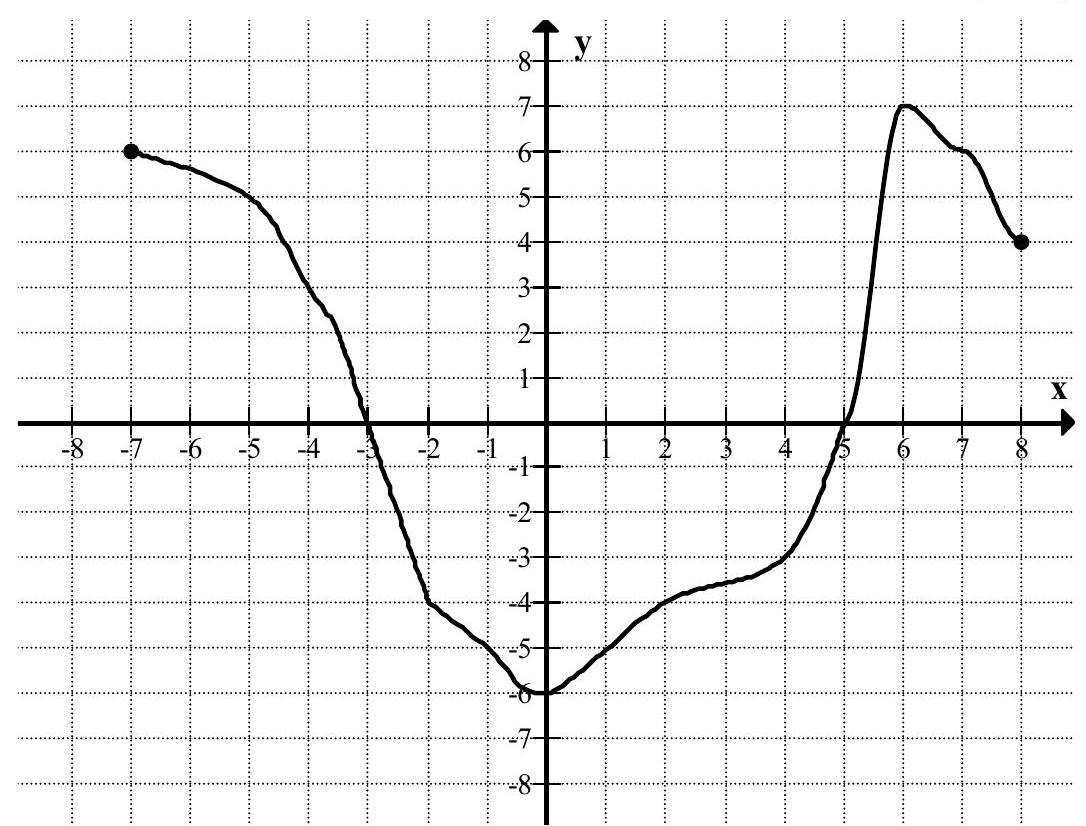
\includegraphics[max width=\textwidth, center]{2024_11_21_e0e8aab895018a50a9a7g-13(2)}

Odczytaj z wykresu i zapisz:\\
a) największą wartość funkcji \(f\),\\

\includegraphics[max width=\textwidth, center]{2024_11_21_e0e8aab895018a50a9a7g-13(1)}\\
b) zbiór rozwiązań nierówności \(f(x)<0\).\\

\includegraphics[max width=\textwidth, center]{2024_11_21_e0e8aab895018a50a9a7g-13}

\begin{center}
\begin{tabular}{|c|l|c|c|}
\hline
\multirow{2}{*}{\begin{tabular}{c}
Wypetnia \\
egzaminator \\
\end{tabular}} & Nr zadania & 28. & 29. \\
\cline { 2 - 4 }
 & Maks. liczba pkt & 2 & 2 \\
\cline { 2 - 4 }
 & Uzyskana liczba pkt &  &  \\
\hline
\end{tabular}
\end{center}

\section*{Zadanie 30. (2 pkt)}
Rozwiąż nierówność \(2 x^{2}-7 x+5 \geq 0\).\\

\includegraphics[max width=\textwidth, center]{2024_11_21_e0e8aab895018a50a9a7g-14}

Odpowiedź:

\section*{Zadanie 31. (2 pkt)}
Wykaż, że liczba \(6^{100}-2 \cdot 6^{99}+10 \cdot 6^{98}\) jest podzielna przez 17 .

\begin{center}
\begin{tabular}{|c|c|c|c|c|c|c|c|c|c|c|c|c|c|c|c|c|c|c|c|c|c|c|c|c|c|c|c|}
\hline
 &  &  &  &  &  &  &  &  &  &  &  &  &  &  &  &  &  &  &  &  &  &  &  &  &  &  &  \\
\hline
 &  &  &  &  &  &  &  &  &  &  &  &  &  &  &  &  &  &  &  &  &  &  &  &  &  &  &  \\
\hline
 &  &  &  &  &  &  &  &  &  &  &  &  &  &  &  &  &  &  &  &  &  &  &  &  &  &  &  \\
\hline
 &  &  &  &  &  &  &  &  &  &  &  &  &  &  &  &  &  &  &  &  &  &  &  &  &  &  &  \\
\hline
 &  &  &  &  &  &  &  &  &  &  &  &  &  &  &  &  &  &  &  &  &  &  &  &  &  &  &  \\
\hline
 &  &  &  &  &  &  &  &  &  &  &  &  &  &  &  &  &  &  &  &  &  &  &  &  &  &  &  \\
\hline
 &  &  &  &  &  &  &  &  &  &  &  &  &  &  &  &  &  &  &  &  &  &  &  &  &  &  &  \\
\hline
 &  &  &  &  &  &  &  &  &  &  &  &  &  &  &  &  &  &  &  &  &  &  &  &  &  &  &  \\
\hline
 &  &  &  &  &  &  &  &  &  &  &  &  &  &  &  &  &  &  &  &  &  &  &  &  &  &  &  \\
\hline
 &  &  &  &  &  &  &  &  &  &  &  &  &  &  &  &  &  &  &  &  &  &  &  &  &  &  &  \\
\hline
 &  &  &  &  &  &  &  &  &  &  &  &  &  &  &  &  &  &  &  &  &  &  &  &  &  &  &  \\
\hline
 &  &  &  &  &  &  &  &  &  &  &  &  &  &  &  &  &  &  &  &  &  &  &  &  &  &  &  \\
\hline
 &  &  &  &  &  &  &  &  &  &  &  &  &  &  &  &  &  &  &  &  &  &  &  &  &  &  &  \\
\hline
 &  &  &  &  &  &  &  &  &  &  &  &  &  &  &  &  &  &  &  &  &  &  &  &  &  &  &  \\
\hline
 &  &  &  &  &  &  &  &  &  &  &  &  &  &  &  &  &  &  &  &  &  &  &  &  &  &  &  \\
\hline
 &  &  &  &  &  &  &  &  &  &  &  &  &  &  &  &  &  &  &  &  &  &  &  &  &  &  &  \\
\hline
 &  &  &  &  &  &  &  &  &  &  &  &  &  &  &  &  &  &  &  &  &  &  &  &  &  &  &  \\
\hline
 &  &  &  &  &  &  &  &  &  &  &  &  &  &  &  &  &  &  &  &  &  &  &  &  &  &  &  \\
\hline
 &  &  &  &  &  &  &  &  &  &  &  &  &  &  &  &  &  &  &  &  &  &  &  &  &  &  &  \\
\hline
 &  &  &  &  &  &  &  &  &  &  &  &  &  &  &  &  &  &  &  &  &  &  &  &  &  &  &  \\
\hline
 &  &  &  &  &  &  &  &  &  &  &  &  &  &  &  &  &  &  &  &  &  &  &  &  &  &  &  \\
\hline
 &  &  &  &  &  &  &  &  &  &  &  &  &  &  &  &  &  &  &  &  &  &  &  &  &  &  &  \\
\hline
 &  &  &  &  &  &  &  &  &  &  &  &  &  &  &  &  &  &  &  &  &  &  &  &  &  &  &  \\
\hline
 &  &  &  &  &  &  &  &  &  &  &  &  &  &  &  &  &  &  &  &  &  &  &  &  &  &  &  \\
\hline
 &  &  &  &  &  &  &  &  &  &  &  &  &  &  &  &  &  &  &  &  &  &  &  &  &  &  &  \\
\hline
 &  &  &  &  &  &  &  &  &  &  &  &  &  &  &  &  &  &  &  &  &  &  &  &  &  &  &  \\
\hline
 &  &  &  &  &  &  &  &  &  &  &  &  &  &  &  &  &  &  &  &  &  &  &  &  &  &  &  \\
\hline
 &  &  &  &  &  &  &  &  &  &  &  &  &  &  &  &  &  &  &  &  &  &  &  &  &  &  &  \\
\hline
 &  &  &  &  &  &  &  &  &  &  &  &  &  &  &  &  &  &  &  &  &  &  &  &  &  &  &  \\
\hline
 &  &  &  &  &  &  &  &  &  &  &  &  &  &  &  &  &  &  &  &  &  &  &  &  &  &  &  \\
\hline
 &  &  &  &  &  &  &  &  &  &  &  &  &  &  &  &  &  &  &  &  &  &  &  &  &  &  &  \\
\hline
 & - &  &  &  &  &  &  &  &  &  &  &  &  &  &  &  &  &  &  &  &  &  &  &  &  &  &  \\
\hline
 & 到 &  &  &  &  &  &  &  &  &  &  &  &  &  &  &  &  &  &  &  &  &  &  &  &  &  &  \\
\hline
 & 到 &  &  &  &  &  &  &  &  &  &  &  &  &  &  &  &  &  &  &  &  &  &  &  &  &  &  \\
\hline
 &  &  &  &  &  &  &  &  &  &  &  &  &  &  &  &  &  &  &  &  &  &  &  &  &  &  &  \\
\hline
 & - &  &  &  &  &  &  &  &  &  &  &  &  &  &  &  &  &  &  &  &  &  &  &  &  &  &  \\
\hline
 & \textbackslash  &  &  &  &  &  &  &  &  &  &  &  &  &  &  &  &  &  &  &  &  &  &  &  &  &  &  \\
\hline
 & - &  &  &  &  &  &  &  &  &  &  &  &  &  &  &  &  &  &  &  &  &  &  &  &  &  &  \\
\hline
 & - &  &  &  &  &  &  &  &  &  &  &  &  &  &  &  &  &  &  &  &  &  &  &  &  &  &  \\
\hline
 & - &  &  &  &  &  &  &  &  &  &  &  &  &  &  &  &  &  &  &  &  &  &  &  &  &  &  \\
\hline
 & - &  &  &  &  &  &  &  &  &  &  &  &  &  &  &  &  &  &  &  &  &  &  &  &  &  &  \\
\hline
 & 到 &  &  &  &  &  &  &  &  &  &  &  &  &  &  &  &  &  &  &  &  &  &  &  &  &  &  \\
\hline
 &  &  &  &  &  &  &  &  &  &  &  &  &  &  &  &  &  &  &  &  &  &  &  &  &  &  &  \\
\hline
 &  &  &  &  &  &  &  &  &  &  &  &  &  &  &  &  &  &  &  &  &  &  &  &  &  &  &  \\
\hline
 &  &  &  &  &  &  &  &  &  &  &  &  &  &  &  &  &  &  &  &  &  &  &  &  &  &  &  \\
\hline
\end{tabular}
\end{center}

\begin{center}
\begin{tabular}{|c|l|c|c|}
\hline
\multirow{2}{*}{\begin{tabular}{c}
Wypelnia \\
egzaminator \\
\end{tabular}} & Nr zadania & \(\mathbf{3 0 .}\) & \(\mathbf{3 1 .}\) \\
\cline { 2 - 4 }
 & Maks. liczba pkt & \(\mathbf{2}\) & \(\mathbf{2}\) \\
\cline { 2 - 4 }
 & Uzyskana liczba pkt &  &  \\
\hline
\end{tabular}
\end{center}

\section*{Zadanie 32. (4 pkt)}
Punkt \(S\) jest środkiem okręgu opisanego na trójkącie ostrokątnym \(A B C\). Kąt \(A C S\) jest trzy razy większy od kąta \(B A S\), a kąt \(C B S\) jest dwa razy większy od katta \(B A S\). Oblicz kąty trójkąta \(A B C\).\\
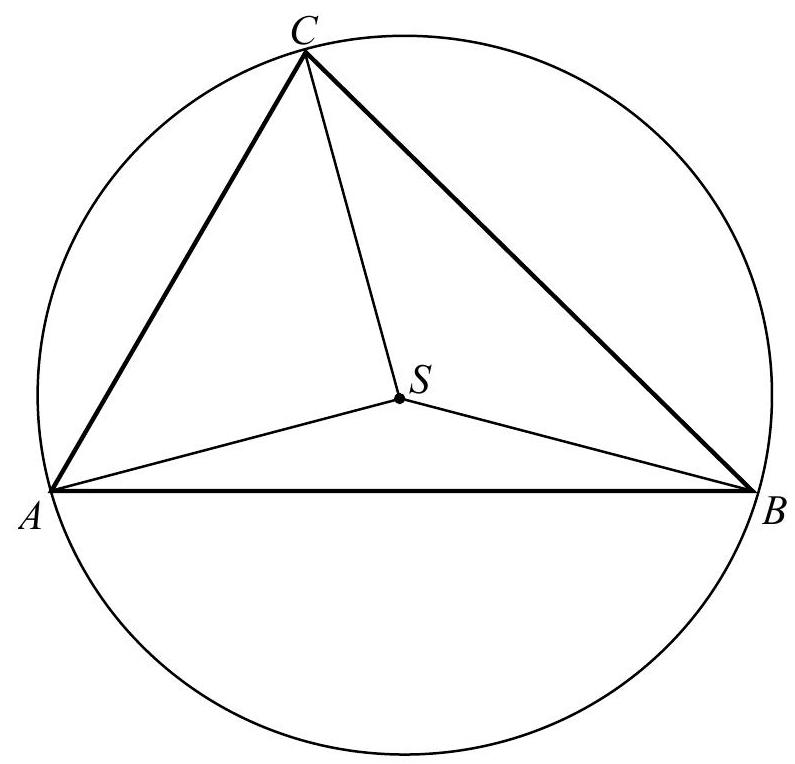
\includegraphics[max width=\textwidth, center]{2024_11_21_e0e8aab895018a50a9a7g-16}

\begin{center}
\begin{tabular}{|c|c|c|c|c|c|c|c|c|c|c|c|c|c|c|c|c|c|c|c|c|c|c|c|c|c|c|c|c|c|}
\hline
 &  &  &  &  &  &  &  &  &  &  &  &  &  &  &  &  &  &  &  &  &  &  &  &  &  &  &  &  &  \\
\hline
 &  &  &  &  &  &  &  &  &  &  &  &  &  &  &  &  &  &  &  &  &  &  &  &  &  &  &  &  &  \\
\hline
 &  &  &  &  &  &  &  &  &  &  &  &  &  &  &  &  &  &  &  &  &  &  &  &  &  &  &  &  &  \\
\hline
 &  &  &  &  &  &  &  &  &  &  &  &  &  &  &  &  &  &  &  &  &  &  &  &  &  &  &  &  &  \\
\hline
 &  &  &  &  &  &  &  &  &  &  &  &  &  &  &  &  &  &  &  &  &  &  &  &  &  &  &  &  &  \\
\hline
 &  &  &  &  &  &  &  &  &  &  &  &  &  &  &  &  &  &  &  &  &  &  &  &  &  &  &  &  &  \\
\hline
 &  &  &  &  &  &  &  &  &  &  &  &  &  &  &  &  &  &  &  &  &  &  &  &  &  &  &  &  &  \\
\hline
 &  &  &  &  &  &  &  &  &  &  &  &  &  &  &  &  &  &  &  &  &  &  &  &  &  &  &  &  &  \\
\hline
 &  &  &  &  &  &  &  &  &  &  &  &  &  &  &  &  &  &  &  &  &  &  &  &  &  &  &  &  &  \\
\hline
 &  &  &  &  &  &  &  &  &  &  &  &  &  &  &  &  &  &  &  &  &  &  &  &  &  &  &  &  &  \\
\hline
 &  &  &  &  &  &  &  &  &  &  &  &  &  &  &  &  &  &  &  &  &  &  &  &  &  &  &  &  &  \\
\hline
 &  &  &  &  &  &  &  &  &  &  &  &  &  &  &  &  &  &  &  &  &  &  &  &  &  &  &  &  &  \\
\hline
 &  &  &  &  &  &  &  &  &  &  &  &  &  &  &  &  &  &  &  &  &  &  &  &  &  &  &  &  &  \\
\hline
 &  &  &  &  &  &  &  &  &  &  &  &  &  &  &  &  &  &  &  &  &  &  &  &  &  &  &  &  &  \\
\hline
 &  &  &  &  &  &  &  &  &  &  &  &  &  &  &  &  &  &  &  &  &  &  &  &  &  &  &  &  &  \\
\hline
 &  &  &  &  &  &  &  &  &  &  &  &  &  &  &  &  &  &  &  &  &  &  &  &  &  &  &  &  &  \\
\hline
 &  &  &  &  &  &  &  &  &  &  &  &  &  &  &  &  &  &  &  &  &  &  &  &  &  &  &  &  &  \\
\hline
 &  &  &  &  &  &  &  &  &  &  &  &  &  &  &  &  &  &  &  &  &  &  &  &  &  &  &  &  &  \\
\hline
 &  &  &  &  &  &  &  &  &  &  &  &  &  &  &  &  &  &  &  &  &  &  &  &  &  &  &  &  &  \\
\hline
 &  &  &  &  &  &  &  &  &  &  &  &  &  &  &  &  &  &  &  &  &  &  &  &  &  &  &  &  &  \\
\hline
 &  &  &  &  &  &  &  &  &  &  &  &  &  &  &  &  &  &  &  &  &  &  &  &  &  &  &  &  &  \\
\hline
 &  &  &  &  &  &  &  &  &  &  &  &  &  &  &  &  &  &  &  &  &  &  &  &  &  &  &  &  &  \\
\hline
 &  &  &  &  &  &  &  &  &  &  &  &  &  &  &  &  &  &  &  &  &  &  &  &  &  &  &  &  &  \\
\hline
 &  &  &  &  &  &  &  &  &  &  &  &  &  &  &  &  &  &  &  &  &  &  &  &  &  &  &  &  &  \\
\hline
 &  &  &  &  &  &  &  &  &  &  &  &  &  &  &  &  &  &  &  &  &  &  &  &  &  &  &  &  &  \\
\hline
 &  &  &  &  &  &  &  &  &  &  &  &  &  &  &  &  &  &  &  &  &  &  &  &  &  &  &  & 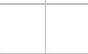
\includegraphics[max width=\textwidth]{2024_11_21_e0e8aab895018a50a9a7g-16(1)}
 &  \\
\hline
 &  &  &  &  &  &  &  &  &  &  &  &  &  &  &  &  &  &  &  &  &  &  &  &  &  &  &  &  &  \\
\hline
 &  &  &  &  &  &  &  &  &  &  &  &  &  &  &  &  &  &  &  &  &  &  &  &  &  &  &  &  &  \\
\hline
 &  &  &  &  &  &  &  &  &  &  &  &  &  &  &  &  &  &  &  &  &  &  &  &  &  &  &  &  &  \\
\hline
 &  &  &  &  &  &  &  &  &  &  &  &  &  &  &  &  &  &  &  &  &  &  &  &  &  &  &  &  &  \\
\hline
\end{tabular}
\end{center}

\begin{center}

\includegraphics[max width=\textwidth]{2024_11_21_e0e8aab895018a50a9a7g-17}
\end{center}

Odpowiedź: \(\qquad\)

\begin{center}
\begin{tabular}{|c|l|c|}
\hline
\multirow{2}{*}{\begin{tabular}{l}
Wypehnia \\
egzaminator \\
\end{tabular}} & Nr zadania & 32. \\
\cline { 2 - 3 }
 & Maks. liczba pkt & 4 \\
\cline { 2 - 3 }
 & Uzyskana liczba pkt &  \\
\hline
\end{tabular}
\end{center}

\section*{Zadanie 33. (4 pkt)}
Pole podstawy ostrosłupa prawidłowego czworokątnego jest równe \(100 \mathrm{~cm}^{2}\), a jego pole powierzchni bocznej jest równe \(260 \mathrm{~cm}^{2}\). Oblicz objętość tego ostrosłupa.\\

\includegraphics[max width=\textwidth, center]{2024_11_21_e0e8aab895018a50a9a7g-18}\\

\includegraphics[max width=\textwidth, center]{2024_11_21_e0e8aab895018a50a9a7g-19}

Odpowiedź:

\begin{center}
\begin{tabular}{|c|l|c|}
\hline
\multirow{2}{*}{\begin{tabular}{l}
Wypelnia \\
egzaminator \\
\end{tabular}} & Nr zadania & 33. \\
\cline { 2 - 3 }
 & Maks. liczba pkt & 4 \\
\cline { 2 - 3 }
 & Uzyskana liczba pkt &  \\
\hline
\end{tabular}
\end{center}

\section*{Zadanie 34. (5 pkt)}
Dwa miasta łaczzy linia kolejowa o długości 336 kilometrów. Pierwszy pociąg przebył tę trase w czasie o 40 minut krótszym niż drugi pociag. Srednia prędkość pierwszego pociagu na tej trasie była o \(9 \mathrm{~km} / \mathrm{h}\) większa od średniej prędkości drugiego pociągu. Oblicz średnią prędkość każdego z tych pociagów na tej trasie.\\

\includegraphics[max width=\textwidth, center]{2024_11_21_e0e8aab895018a50a9a7g-20}\\

\includegraphics[max width=\textwidth, center]{2024_11_21_e0e8aab895018a50a9a7g-21}

Odpowiedź:

\begin{center}
\begin{tabular}{|c|l|c|}
\hline
\multirow{2}{*}{\begin{tabular}{l}
Wypehnia \\
egzaminator \\
\end{tabular}} & Nr zadania & 34. \\
\cline { 2 - 3 }
 & Maks. liczba pkt & 5 \\
\cline { 2 - 3 }
 & Uzyskana liczba pkt &  \\
\hline
\end{tabular}
\end{center}

\section*{BRUDNOPIS}

\end{document}